% My Dissertation in TeX

\documentclass{article} %\documentclass{IEEEtran}

% Packages
\usepackage{setspace}
\usepackage{amsmath}
\usepackage{graphicx}

% Bibliography Package and Style
\usepackage{natbib}
%\bibliographystyle{jmr}
\bibliographystyle{agsm}

%\usepackage[style=numeric,citestyle=alphabetic,bibstyle=authortitle]{biblatex}

\title{Investigating the Impact of AI Techniques on Inter-Flock Dynamics}
\date{2019-02-17}
\author{Matt Hunter}

% This acts as a container - Works like a pragma region basically
% document is a key word, meaning you must have it containing the whole document
\begin{document}

% gobble - no numbers
% arabic - arabic numbers (1, 2, 3, 4, etc.)
% roman - roman numbers (i, ii, iii, iv, etc.)
\pagenumbering{gobble} 

% produce a title page
\maketitle
\newpage

% Set the initial page numberings to roman numerals to separate page numberings
\pagenumbering{roman}
\doublespacing

	\tableofcontents
	
	\listoffigures
	\listoftables

\newpage
\pagenumbering{arabic} 
\singlespacing

	%!TeX root=Main Document/Dissertation.tex

\begin{center}
\Large\textbf{Abstract}
\end{center}

\paragraph{Context}
Flocking algorithms represent a kind of group behaviour that collectively improves the survival chances of individual members, and using genetic algorithms to improve a flock is an area already under exploration. However, not so looked into is the ability of a genetic algorithm to improve a flocks competitiveness versus a regular flocking algorithm and the changes in behaviours that may result.

\paragraph{Aim}
To develop an environment in which a flock that improves over generations via a genetic algorithm can compete over resources with a regularly implemented flock, using the expanded boids model. Exploring how the genetic algorithm affects the competitiveness of the flock in the environment in survival, potential convergence in evolutionary traits, and emergent situational behaviours.

\paragraph{Method}
A competitve environment with a limited resource pool not suitable to sustain two flock populations was developed. For this environment a flocking algorithm and genetic algorithm were developed. 

\paragraph{Results}


\paragraph{Conclusion}


%\begin{abstract}
%\end{abstract}


	%\paragraph{Context}
	%Artificial intelligence is a rapidly expanding field, there is a clear useful context in their use in Flocking Techniques.
	
	%\paragraph{Aim}
	%Investigate the impact of AI techniques on the dynamic interaction of flocks with each other to see if this has a beneficial effect in comparision to regular flocking algorithms.
	
	%\paragraph{Method}
	%Using an application that models flocking behaviour (developed by the author), observe and compare AI flocking strategies to those of regular flocking algorithms. This will be developed using the AI techniques found to be most likely to produce viable intelligent flocking behaviour.
	
	%\paragraph{Results}
	%The analysis of the effectiveness of strategies that the AI come up with in their interactions with other flocks, with contrast and comparison to the behaviour of standard flocking algorithms.
	
	%\paragraph{Conclusion}
	%This project will display the flocking strategies that emerge in their interactions with other flocks, and conclude on their effectiveness in relation to other strategies and flock type. This will demonstrate the impact the AI techniques have on this kind of flocking interaction.

	
\newpage

	%!TeX root=Main Document/Dissertation.tex

\section{Introduction}

\subsection{General Introduction and Background Information} % May not be entirely necessary to title this this way and can probably be skipped (depends how you write this though!)

Flocking is an emergent property of social behaviours, it is the common movement of individuals guided by both social and environmental influences, and is one in which many social organisms engage. These flocks of organisms can be found interacting with other flocks in nature, and the way they interact is as varied as it is interesting.

Producing flocking behavior that recreates those found in nature is an endeavor already undertaken and in constant update. The field, taking off in 1987 with Craig Reynolds’ influential paper \citep{Reynolds:1987:FHS:37402.37406}, shows how realistic flocking behaviour can already be achieved by applying 3 simple rules to each boid (‘boid’ as coined in the prior paper, this is essentially an agent) in regard to its neighbours: Cohesion, movement toward the average position; Alignment, movement toward the average direction; and Separation, movement to avoid collision. 

Since then, the original flocking algorithm has been extended in various ways, with communication techniques, mathematical models for how leadership arises in the flock, as well as models for how consensus is made in a flock. These expansions allow for more complex behaviours and reactions to the enviornment and surroundings.

Learning behaviours have also been added. The behaviour and strategies flocks produce are patterns. This means if a flock can learn and understand those patterns it has a significant advantage over that other flock – an interesting example would be a group of honey hunters and smoke; bees flee the nest if they think there is a fire, the first warning sign to this is smoke, as a group (or flock) they take advantage of this by releasing smoke into the hive. The bees evacuate the nest; they get honey. 

This dissemination of new knowledge, either through behaviour or communication is interesting because it can increase the complexity of the reactions the flock has to a given situation. This added complexity may lead to new behaviours that may not have been easily predicted or thought of as something a flock could produce. 



\subsection{Aim, Objectives and Research Question} 
\paragraph{Aim}To investigate if a flock improved by a genetic algorithm can outcompete a regular flock in a competitive environment, and to identify what changes the genetic algorithm produces, convergences and the kinds of behaviours produced over time.

\paragraph{Objectives} % These objectives need to be updated as they are not reflective of the project in its current form
\begin{itemize}
\item % This item especially needs updating!
To research and evaluate AI techniques, studying their relevance and potential for further development in applying them to flocking algorithms, with particular focus on artificial life techniques. 
\item
To produce an application that models flocking behaviour, and allows the observation and comparison of AI flocking strategies to regular flocking algorithms. This will be developed using the prior identified AI techniques most likely to produce viable flocking behaviours. 
\item
To analyse the effectiveness of strategies that the AI come up with in their interactions with other flocks, comparing and contrasting that to the behavior of standard flocking algorithms.
\end{itemize}

\paragraph{Research Question}
What impact can a genetic algorithm have on the dynamic interaction of flocks with each other in comparison to that of regular flocking techniques?




\newpage

	%!TeX root=Main Document/Dissertation.tex

% Protip - Have you made a statement, would you consider it a fact? Back it up with a reference! (unless its 'common sense' ~ Spooky)

% Also you can expand the number of references you have by stacking references with similar conclusions to the ones you have already 
% cited in your text. This will only add to the confidence one can have in the assertion.

\section{Literature Review}

\subsection{Flocking in Nature - Swarm Behaviour}
Flocking algorithms draw a lot of their inspiration from the behaviour of flocks in the natural world \citep{flake1998computational}. As there are many examples of this behaviour in organisms across the planet, there is a lot of information and insight that can be gleaned on how to design these algorithms. Flocks are included in the field of Swarm Behaviour, that is, the study of swarms in the natural world 

	\paragraph{Decision Making}
	The way decisions are made in a flock emerges is varied. The two main ways are via consensus and leadership. An interesting look at this can be found in the behaviour of pigeons. A study conducted into the behaviour of these birds in a flock \citep{Jorge2414} found that leadership initially emerged from younger pigeons in the flock, but as the flight went on older members of the flock led the group, the paper then goes on to discuss how social versus personal information affects the behaviour of the flock. What this displays, is how the extra experience of older members of the flock is taken advantage of in determining leadership and therefore the actions they take as a flock, in this way they build consensus on their leadership through the choices individual flock members make in their group. This is further confirmed in \textit{ 'Misinformed leaders lose influence over pigeon flocks' }\citet{doi:10.1098/rsbl.2016.0544}. What this displays is the interaction between consensus and leadership in making decisions, and demonstrates that they can both be present in the process.
	
	% Here we can mention eusocial insects and their very dominant hierarchy (e.g. Queens of the hive/nest) Queens can be picked though! This may be interesting to explore
	% The main thing we can explore here is consensus vs leadership
	\paragraph{Eusocial Behaviour}
	While not specifically flocking as it pertains to biology, this falls under the bracket of swarm behaviour and has interesting relationships which can inform us on how to expand flocking algorithms in beneficial ways. For example, communication can occur in a variety of ways; ants use pheromones to find shortest paths \citep{DORIGO199773}; bees use a waggle dance % Expand on this from here...
	
	\paragraph{Dynamic Adaptation to Environmental Pressures}
	
	
	%\paragraph{The path from subsocial to eusocial behaviour}
	% This could be a potentially interesting path to go down here in terms of how it would relate to the evolution in genetic algorithms and potential first steps the genetic algorithm should take in terms of its path towards smart flocking behaviour
	
	
	
	\paragraph{Why this is relevant}
	This is relevant as it inspires the work done in flocking algorithms and the work of similar fields, which has influence on the design of said algorithms. 


\subsection{Flocking Algorithm}
Flocking algorithms draw inspiration from the natural world, however the design of these algorithms involves mathematical approximations of the behaviours involved, the interactions that take place and the systems overall.

	\paragraph{Reynolds Boids}
	In the often cited paper when it comes to discussions of flocks: \textit{'Flocks, herds and schools: A distributed behavioral model'} \citet{Reynolds:1987:FHS:37402.37406}, we see that we have the three main forces that make up a basic flock: Separation, Cohesion and Alignment. These are approximative forces that represent the aggregate motion of a collection of boids (representing flock members, which in turn can represent different species in nature).
	
	\paragraph{Expanded Boids} % Potential for adding relevant equations here but they may be more relevant to be placed in the method
	
	
	\paragraph{Decision Making}
	
	
	\paragraph{Learning and Curiosity}
	
	

\subsection{The Interaction of Flocking Algorithms}
In the paper \textit{'Simulating Species Interactions and Complex Emergence in Multiple Flocks of Boids with GPUs'} \citet{husselmannsimulating}


\subsection{Genetic Algorithm}


\subsection{The Effect of AI on Flocking Algorithms}




\subsection{The Interaction of an AI Flock with another Flock}













\newpage

	%\input{../Method}

\newpage
	
	%

	\section{Notes}

	This is an example of a citation in text:	\cite{Reynolds:1987:FHS:37402.37406}.\\
	This is an example of a citation in brackets \citep{Reynolds:1987:FHS:37402.37406}.

	\begin{figure}
		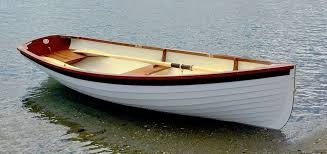
\includegraphics[width=\linewidth]{../Images/boat.jpg}
		\caption{A Boat.}
		\label{fig:boat1}
	\end{figure}
	
	Figure \ref{fig:boat1} shows a boat.
		
	% Example 1:
	\ldots when Einstein introduced his formula
	\begin{equation}
		e = m \cdot c^2 \; ,
	\end{equation}
	which is at the same time the most widely known and the least
	well understood physical formula
	
	% Example 2:
	\ldots from which follows Kirchoff's current law:
	\begin{equation}
		\sum_{k=1}^{n} I_k = 0 \; ,
	\end{equation}
	Kirchoff's voltage law can be derived \ldots
	
	% Example 3:
	\ldots which has several advantages.
	\begin{equation}
		I_D = I_F - I_R
	\end{equation}
	is the core of a very different transistor model. \ldots
	
	\begin{equation}
		f(x) = x^2
	\end {equation}
	
	\begin{equation*}
		3+ 3 = 6
	\end {equation*}
	\begin{equation*}
		1 = 5 - 4
	\end {equation*}
	
	\begin{align*}
	% The ampersand identifies where the equations will align
		1 &= 5 - 4\\ % In this case the \\ indicates a new line
		3+ 3 &= 6\\ 
		\\
		f(x) &= x^2\\
  		g(x) &= \frac{1}{x}\\
  		F(x) &= \int^a_b \frac{1}{3}x^3
	\end {align*}

\newpage

	\bibliography{../Bibliography/bibliography}

	% An alternative formatting for if it seems better to place these at the end of the document
	%\begin{appendix}
	%	 \listoffigures
	%	 \listoftables
	%\end{appendix}
	
\end{document}